\documentclass{instructions}

\usepackage{xspace}

\newcommand{\git}{\texttt{git}\xspace}
\newcommand\bs{\char`\\}

\title{Practical 3: Humanoid robots}
\date{\today}

\summary{
Head first in humanoid robot programming! This practical last three weeks: this
week, you will learn how to program the Aldebaran's Nao robot, using the
Choregraphe IDE. Week 2 and 3 will focus on Plymouth's Drake robot: up to you to
get it to walk!}

\objectives{
At the end of these 3 sessions, you should have achieved the following targets:

\begin{itemize}
    \item Let Nao recognising simple verbal commands (programmed in Choregraphe);
    \item Link verbal commands to let the robot walk or change direction (programmed in Choregraphe);
    \item Reflect on the walking implemented on the Nao;
    \item Implement a small demonstration on the Nao using a range of different behaviours in Choregraphe;

    \item Set-up and initialise the Drake robot;
    \item Try a range of difference gait parameters and assess their impact on the walking behaviour;
    \item Let the robot walk towards a visual target;
    \item Let the robot walk five meters on the red tape without assistance from a human handler.

\end{itemize}
}

\begin{document}

\maketitle


\note{

    This practical is \textbf{not} assessed. We do not ask you to submit any
    report.

    Please note however that \textbf{you are required to attend all the laboratory
    practical sessions}.
}


%%%%%%%%%%%%%%%%%%%%%%%%%%%%%%%%%%%%%%%%%%%%%%%%%%%%%%%%%%%%%%%%%%%%%%%%%%%%%%%%%%%%%%%%%%

\intro

We have 6 Nao robots. Please form groups of 3-4 people per robot.

\part{Week 1: Nao programming}

\begin{center}
    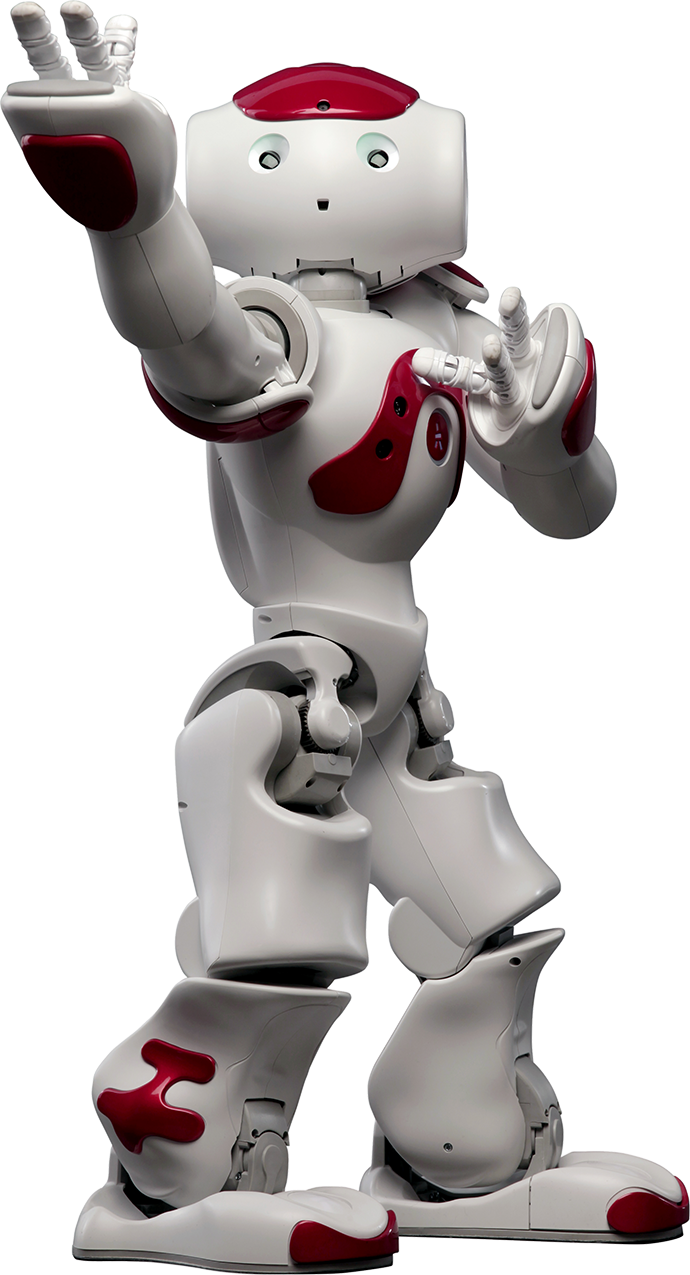
\includegraphics[width=0.3\linewidth]{figs/nao}
\end{center}

\step{Install Choregraphe}

You can use the USB stick that we have prepared for you.

Make sure you can successfully connect to the robot.

\step{Programming challenges}

Create programs to get the robot to:

\begin{enumerate}
    \item say ‘Hello World’
    \item ask a question, and to wave if you answer 42
    \item walk while being verbally guided (‘forward’, ‘backward’, ‘left’, ‘right’)
\end{enumerate}

\note{You can find Choregraphe's documentation on Aldebaran website or on the
DLE.}

\step{Mini project: design a multi-modal interaction with the robot}

Within the remaining time, create a more engaging interaction with your robot.

Explore the available capabilities of the robot; feel free to use custom Python
code if you need to; impress us!

Examples:

\begin{itemize}
    \item The robot greets and follows any face it detects
    \item Adventure story-telling where the human decides “what comes next”
    \item ...up to you!
\end{itemize}

Make a 2 mins video of your mini-project, upload it on YouTube and submit the
link on the DLE to showcase it!

\part{Weeks 2 \& 3: Plymouth Drake robot}

\begin{center}
    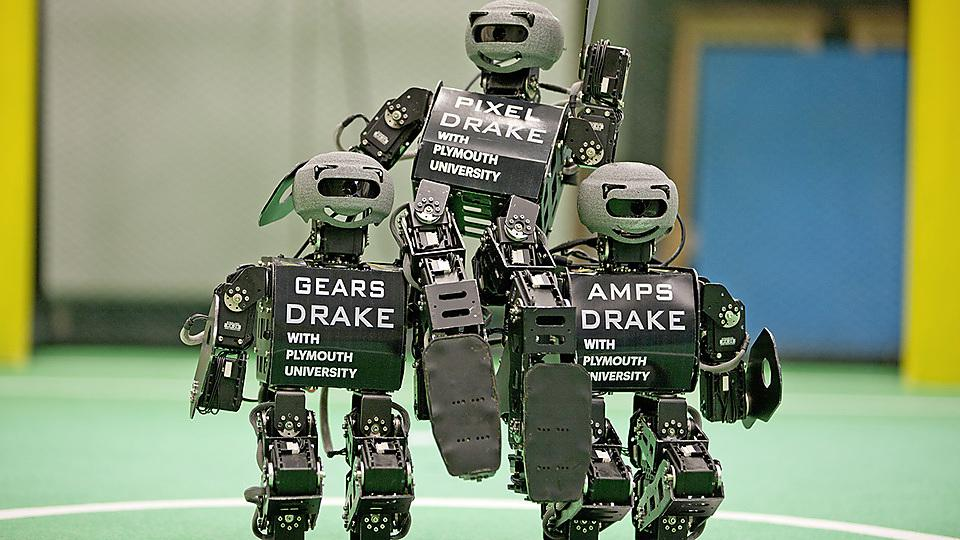
\includegraphics[width=0.9\linewidth]{figs/drake}
\end{center}

For this practical, please download and open
\href{https://dle.plymouth.ac.uk/mod/equella/view.php?id=471210}{the Drake robot
manual} on the DLE.
\end{document}
